\documentclass[../../Aurora C# unofficial manual.tex]{subfiles}

\begin{document}
	\section{Modifying stars}\label{1_modifying_stars}
	Original post can be found
	\href{http://aurora2.pentarch.org/index.php?topic=8495.msg118725#msg118725}{here}.
	\\\\
	
	C\# Aurora allows you to manipulate star systems in SM Mode. While it would be difficult to design a system during the original generation process, due to the complexities involved, you can now add or modify stars and system bodies. This post covers modifying stars.
	
	You click on a star in the System View and then click Change Star. The dialog below pops up and allows you to select spectral class, orbital distance, bearing and parent star.
	\begin{figure}[h]
		\centering
		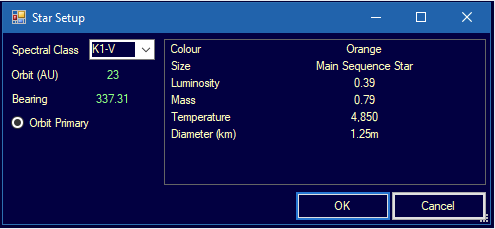
\includegraphics[width=0.5\linewidth]{images/StarSetup}
		\caption[Star Setup]{Star Setup}
		\label{fig:starsetup}
	\end{figure}
	Here is an example from my current test campaign that changes the B component of Alpha Centauri from a K1-V star to an F0-V, which is much hotter. The star will orbit more quickly due to the increased mass, plus all the planets orbiting the star are affected by the increased mass and luminosity of the different star. Temperatures will change, along with potentially hydrosphere type and atmospheric composition (as gases freeze out or boil). Oceans or ice sheets may convert entirely to water vapour given a significant temperature rise. Planets may change their tide-locked status.
	\begin{figure}[H]
		\centering
		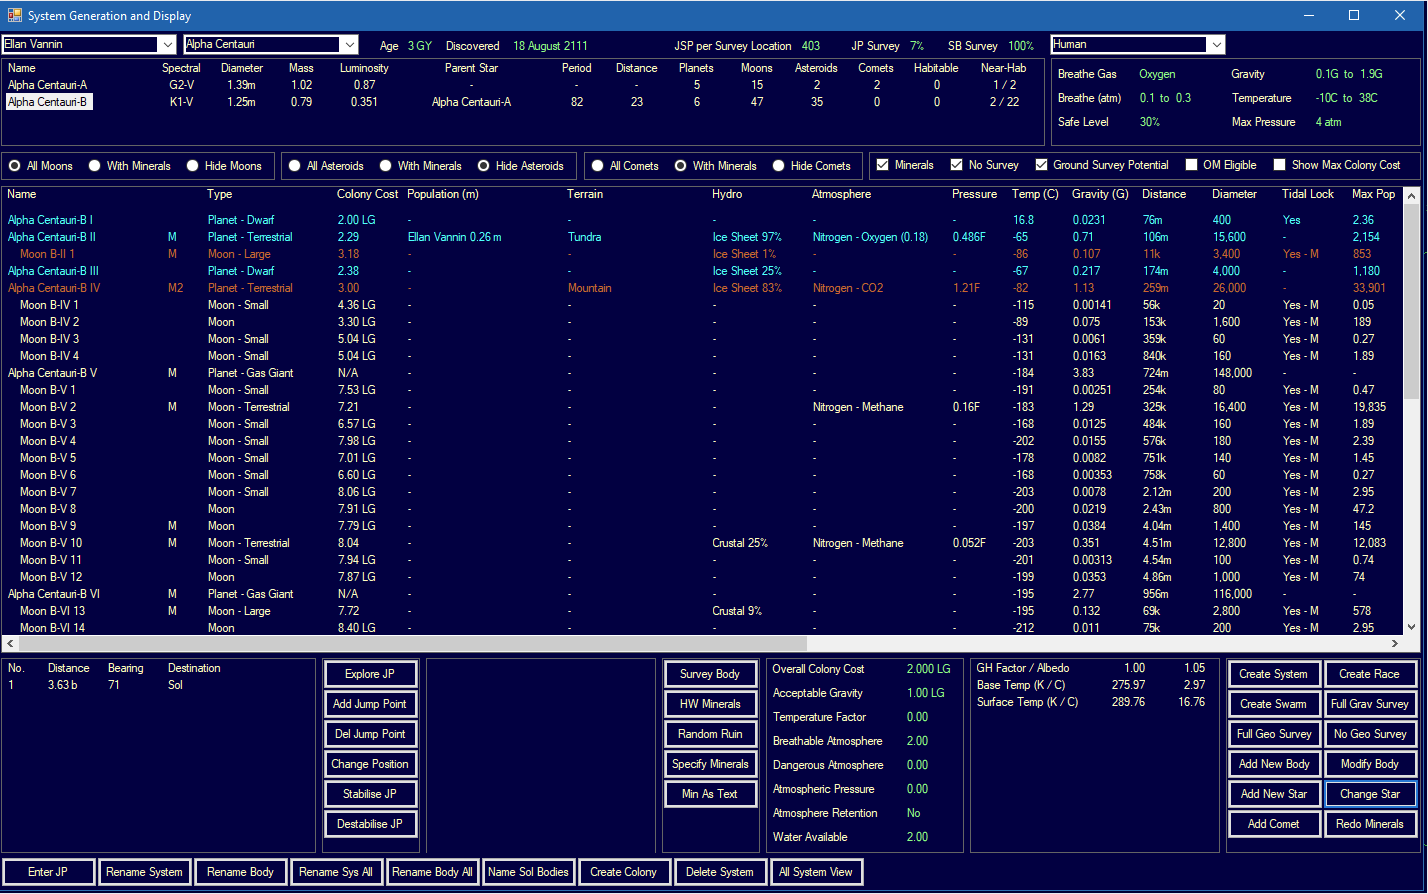
\includegraphics[width=0.95\linewidth]{images/StarSetupExample}
		\caption[Star Setup Example]{Star Setup Example 1}
		\label{fig:starsetupexample}
	\end{figure}
	\begin{figure}[H]
		\centering
		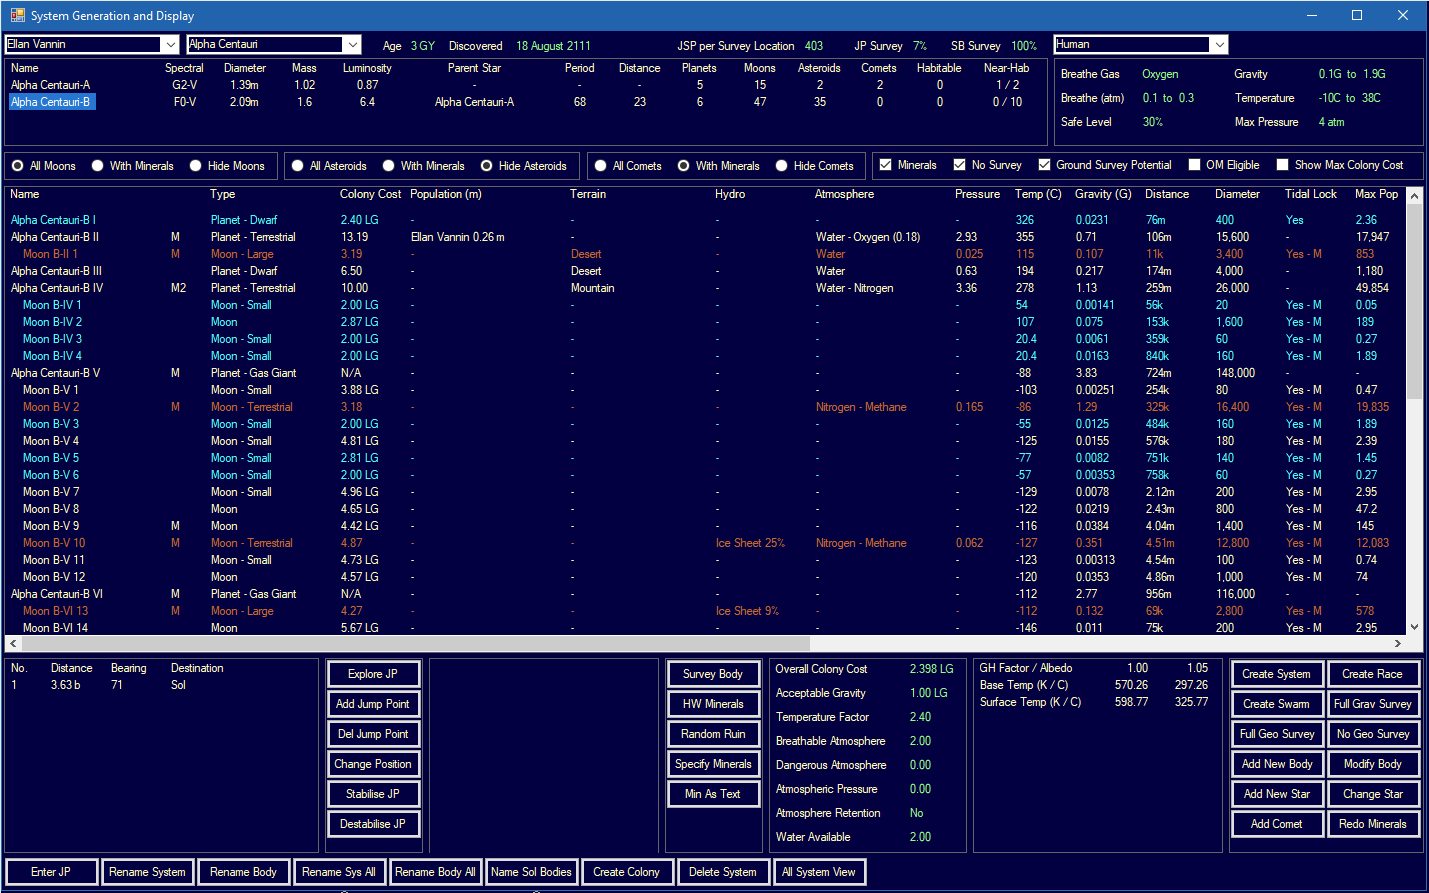
\includegraphics[width=0.95\linewidth]{images/StarSetupExample2}
		\caption[Star Setup Example 2]{Star Setup Example 2}
		\label{fig:starsetupexample2}
	\end{figure}
	
	These two screenshots show the effect of moving the star further from the primary.
	\begin{figure}[H]
		\centering
		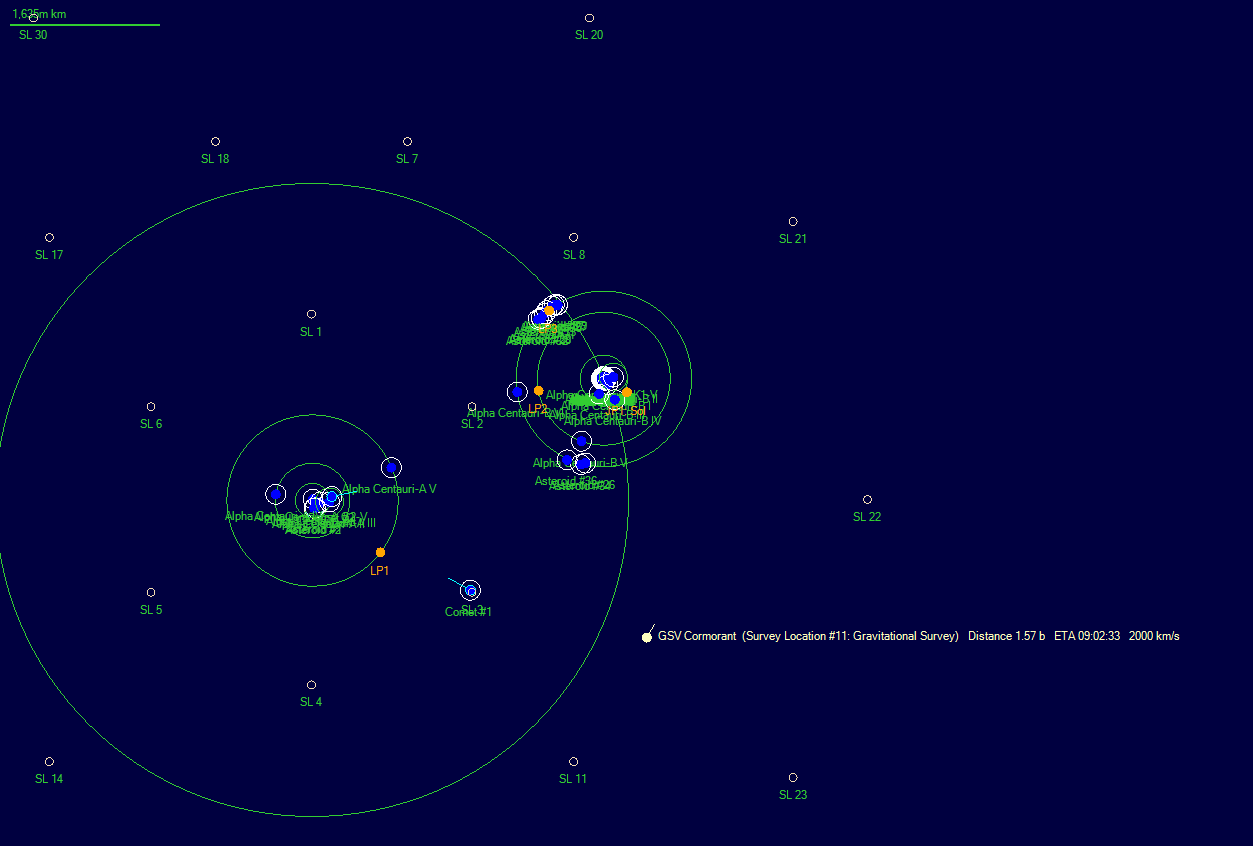
\includegraphics[width=0.95\linewidth]{images/Engineering003}
		\caption[Engineering Example]{Engineering Example 1}
		\label{fig:engineering003}
	\end{figure}
	\begin{figure}[H]
		\centering
		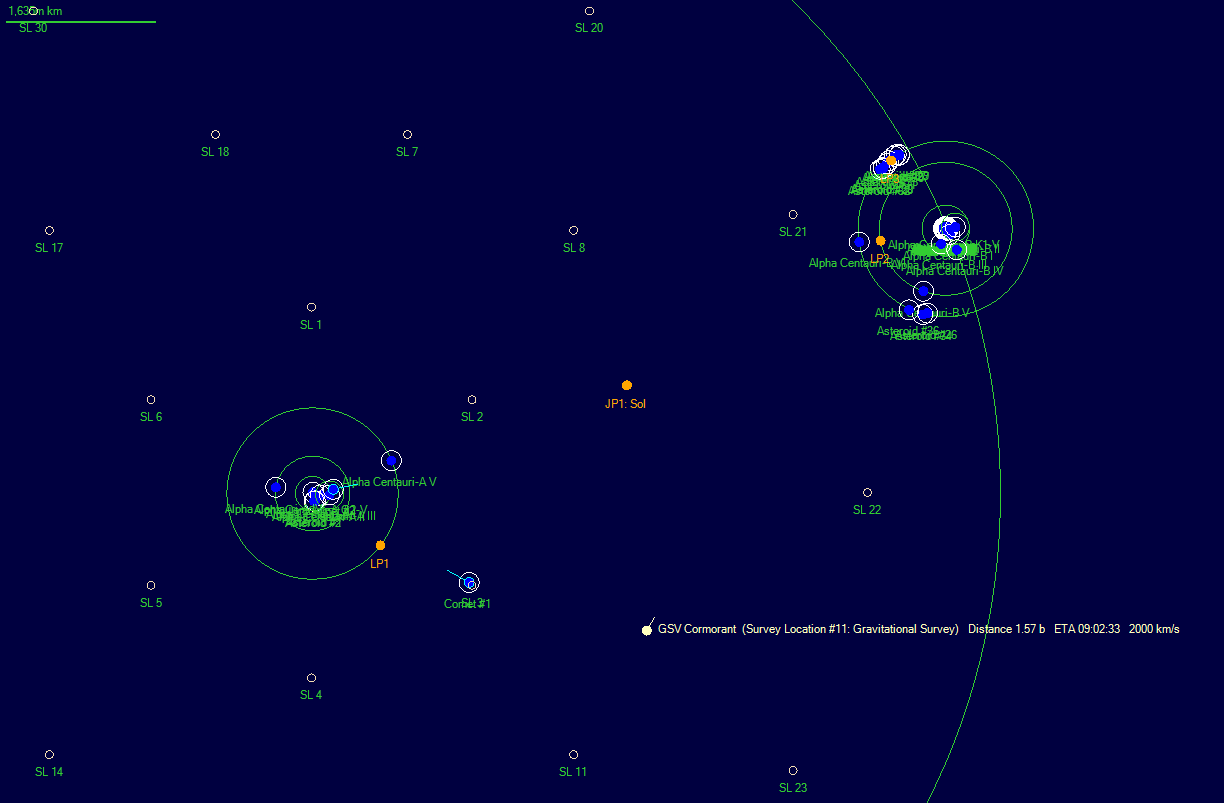
\includegraphics[width=0.95\linewidth]{images/Engineering004}
		\caption[Engineering Example 2]{Engineering Example 2}
		\label{fig:engineering004}
	\end{figure}
\end{document}